\chapter{Appendix 1}\label{app1}


\section{Explanation of Various Consensus Algorithms}

\subsubsection{Proof of Work}
PoW works by each node having to show it performed an amount of computationally difficult work, such as mathematical puzzle such as finding a specific hash, and which ever node finds it first is allowed to form the next block and place in it the transactions that it has received. This action is called mining.\cite{nakamoto2012bitcoin}

This method works well when there are many participants in the network but has the drawbacks of using a lot of computing power and electricity which can create a barrier to participating in the consensus process. For example mining in the Bitcoin network now is unfeasible on a regular computer, requiring ASIC(Application Specific Integrated Circuit) devices to participate. They also have very slow confirmation times.\cite{Baliga2017UnderstandingBC} 

\subsubsection{Proof of Stake(PoS)}
PoS works by instead of proving that a node has spent time working on a cryptographic puzzle, they provide some of their cryptocurrency as a stake, which allows the node to vote on a correct block to be added to the ledger. By having a stake, nodes are discouraged from acting maliciously as if they do they will have their stake taken, and lose more than they gain from their actions. The algorithm pseudo-randomly selects a validator from the pool of validators, removing the ability for validators to be able to guess their turn.\cite{buterin2014ethereum}

PoS has the benefits of not requiring ASIC devices in order to compete in the consensus process, but instead requiring a non insignificant sum of cryptocurrency. It also doesn't require large amounts of electricity which is a cost and environmental benefit. 

\subsubsection{Proof of Elapsed Time(PoET)}
PoET works by using a Trusted Execution Environment(TEE), the TEE running on each participating node, each node then requests a wait time from the TEE. Then the node with the shortest wait time wins and is allowed to commit the next block to the chain. The TEE ensures that wait time cannot be modified and each nodes wait time is randomized. 

The drawback of PoET is the requirement of using a TEE, which must be run on specialized hardware like Intel's SGX.\cite{Linux2018Intro}

\subsubsection{Byzantine Fault Tolerance(BFT) and Crash Fault Tolerance(CFT)}
These consensus protocols work on permissioned blockchains and make use of trust between participants, removing the need for economic incentive for miners, needed in protocols like PoW and PoS. They work by having certain trusted nodes and select a leader among them to achieve consensus. In a network of N nodes, CFT can tolerate up to 2/N nodes failing, but does not assume the presence of a malicious actor, while BFT can tolerate up to 2/N nodes failing or acting malicious.

\section{Making ARM64 Binaries and Images}

\begin{figure}
    \centering
    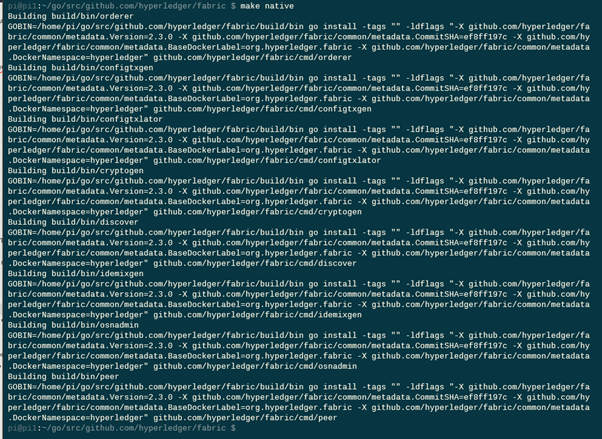
\includegraphics{images/makenative.png}
    \caption{Output of make native}
    \label{fig:my_label}
\end{figure}


\begin{figure}
    \centering
    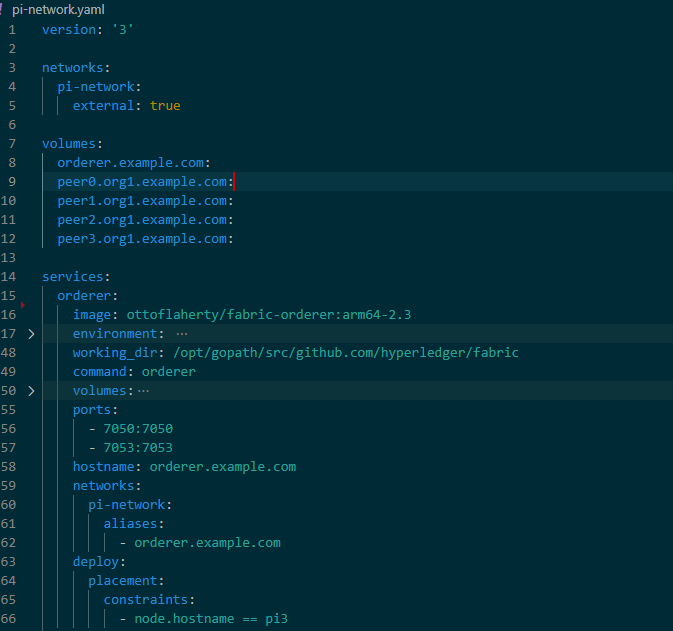
\includegraphics[width=\textwidth]{pinetwork1.PNG}
    \caption{Caption}
    \label{fig:my_label}
\end{figure}

\begin{figure}
    \centering
    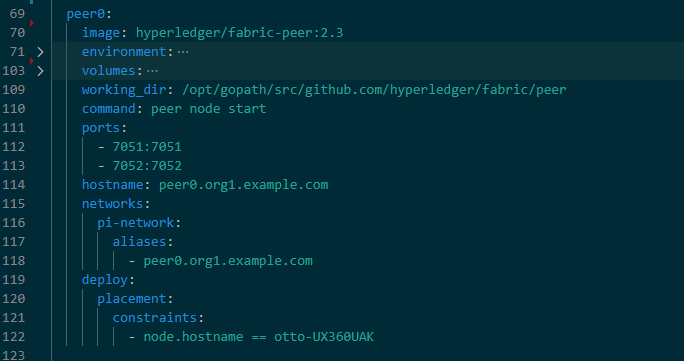
\includegraphics[width=\textwidth]{pinetwork2.PNG}
    \caption{Caption}
    \label{fig:my_label}
\end{figure}

\begin{figure}
    \centering
    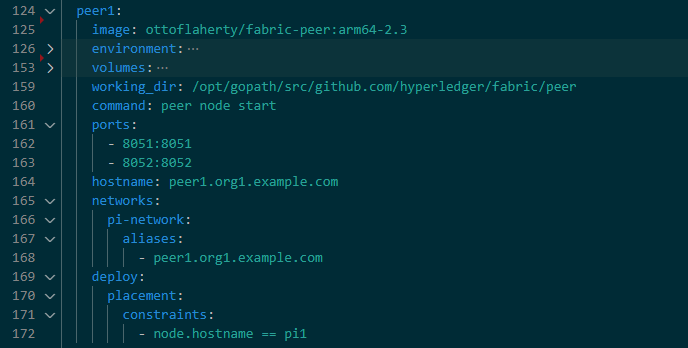
\includegraphics[width=\textwidth]{pinetwork3.PNG}
    \caption{Caption}
    \label{fig:my_label}
\end{figure}
\begin{figure}
    \centering
    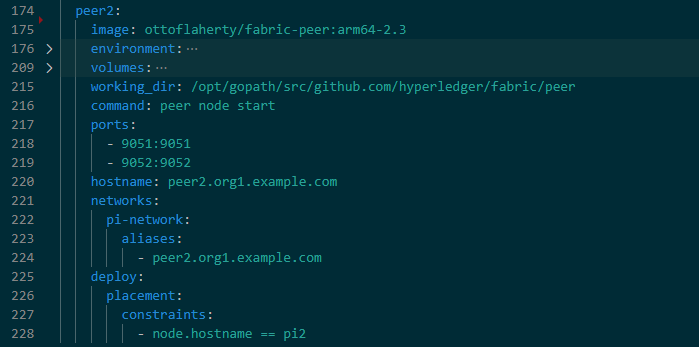
\includegraphics[width=\textwidth]{pinetwork4.PNG}
    \caption{Caption}
    \label{fig:my_label}
\end{figure}